% !TEX root = knottedMain.tex
\documentclass[varwidth=\maxdimen]{standalone}

\usepackage{mathtools,amssymb,mathrsfs,dutchcal,upgreek,faktor,accents,etoolbox,multicol}
\usepackage[dvipsnames]{xcolor}
\definecolor{mygreen}{RGB}{	8,156,79 }
\usepackage{tikz,tikz-cd}
\usetikzlibrary{patterns,knots,arrows.meta,decorations.markings}
\tikzset{>={Straight Barb[scale=0.85]}}
\tikzcdset{
  cells={font=\everymath\expandafter{\the\everymath\displaystyle}},
  arrow style=tikz,
  diagrams={>={Straight Barb[scale=0.85]}},
  every label/.append style = {font = \small}
}


\begin{document}
\begin{tabular}{@{}c@{}}
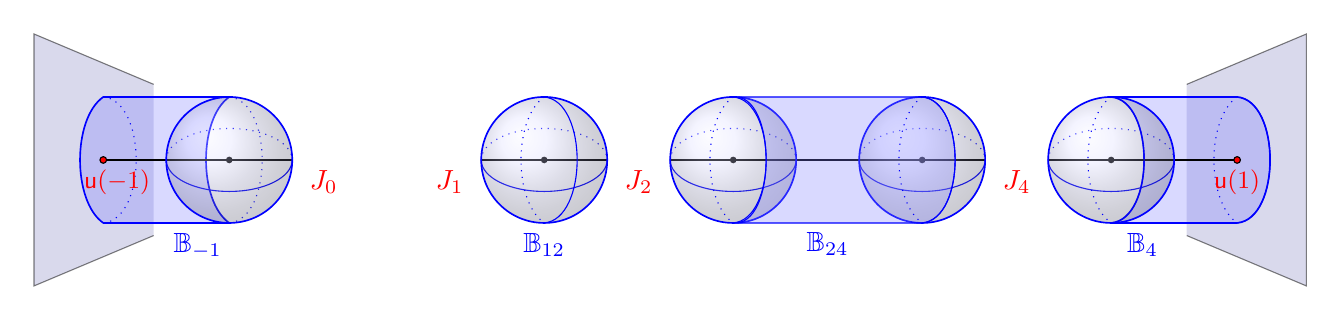
\begin{tikzpicture}[scale=0.8]
    \clip (-2.2,-2.1) rectangle (18.2,2.1);
    % boundary of M
    \fill[blue!50!black,opacity=0.15,draw=black,draw opacity=0.5]
        (16.2,-1.2) -- (18.1,-2) -- (18.1,2) --  (16.2,1.2) ;
    \fill[blue!50!black,opacity=0.15,draw=black,draw opacity=0.5]
        (-0.2,1.2) -- (-2.1,2) -- (-2.1,-2) -- (-0.2,-1.2) ;
    % cylinder left
    \fill[draw=blue,semithick,fill=blue!50!white,fill opacity=0.3]
        (-1,-1) -- (1,-1) to[out=145,in=-145, distance=0.6cm] 
        (1,1) -- (-1,1) to[out=-145,in=145, distance=0.6cm] (-1,-1);
    \draw[semithick,blue] 
        (-1,1) -- (1,1) 
        (1,-1) -- (-1,-1);
    % vertical arcs on the first sphere
    \foreach \x in {-1,1}{
        % \draw[blue,semithick]
        %     (\x,1) to[out=-145,in=145, distance=0.6cm] (\x,-1);
        \draw[blue, dotted]
            (\x,1) to[out=-5,in=5, distance=0.7cm] (\x,-1);
    }
    % right cylinder
    \fill[draw=blue,semithick,fill=blue!50!white,fill opacity=0.3]
        (15,1) -- (17,1) to[out=-5,in=5, distance=0.7cm] 
        (17,-1) -- (15,-1) to[out=5,in=-5, distance=0.7cm] (15,1);
    % old
    \draw[semithick]
        (-1,0) -- (2,0)
        node[pos=0.5, below=0.8cm,blue]{$\mathbb{B}_{-1}$}
        (5,0) -- (7,0) node[pos=0.5, below=0.8cm,blue]{$\mathbb{B}_{12}$}
        (8,0) -- (10,0)  -- (11,0)   -- (13,0)
        (14,0) -- (17,0) node[pos=0.5, below=0.8cm,blue]{$\mathbb{B}_{4}$} ;
    \draw[thick, red]
        (2.5,0) node[below]{$J_{0}$}
        (4.5,0) node[below]{$J_{1}$}
        (7.5,0) node[below]{$J_{2}$}
        (13.5,0) node[below]{$J_{4}$}
        % (16.5,0) node[below]{$J_{5}$}
        ;
    % \draw[mygreen, thick]
    %     (0,0) -- (2,0) node[fill=mygreen!20,draw, pos=0.5]{}
    %     (1, 0) node[below=2pt]{$J_0$};
    \foreach \y/\ytext in {1/0,6/1,9/2,12/3,15/4}{
        \fill[fill=black] (\y,0) circle (1.5pt) 
        % node[below]{\small$u_{\ytext}$} 
        ;
    }
    %spheres
    \foreach \y in {1,6,9,12,15}{
        \draw[blue] (\y-1,0) arc (180:360:1cm and 0.5cm);
        \draw[blue,dotted] (\y-1,0) arc (180:0:1cm and 0.5cm);
        \shade[ball color=blue!20!,opacity=0.3] (\y,0) circle (1cm);
        \draw[blue,semithick] (\y,0) circle (1cm);
    }
    % blue cylinder
    \fill[draw=blue,fill=blue!50!white,fill opacity=0.3]
        (9,1) -- (12,1) to[out=-5,in=5, distance=0.7cm] (12,-1) -- (9,-1) to[out=-5,in=5, distance=0.7cm] (9,1);
    \draw[color=blue] (10.5, -1) node[below]{$\mathbb{B}_{24}$};
    % vertical arcs
    \foreach \x in {6,9,12,15,17}{
        \draw[blue]
            (\x,1) to[out=-5,in=5, distance=0.7cm] (\x,-1);
        \draw[blue,dotted]
            (\x,1) to[out=-145,in=145, distance=0.6cm] (\x,-1);
    }
    % \foreach \y in {0,2}{
    %     \fill[mygreen,draw=black,semithick] (\y,0) circle (1.5pt);
    % }
    \fill[red,draw=black]
        (-1,0) circle (1.5pt) (-0.78,0) node[below]{\small$\mathsf{u}({-}1)$}
        (17,0) circle (1.5pt) node[below]{\small$\mathsf{u}(1)$};
\end{tikzpicture}

\\

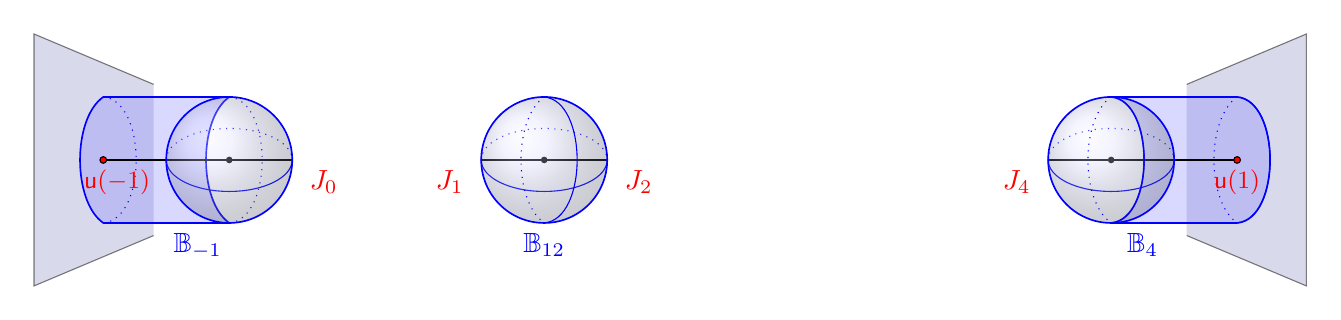
\begin{tikzpicture}[scale=0.8]
    \clip (-2.2,-2.1) rectangle (18.2,2.1);
    % boundary of M
    \fill[blue!50!black,opacity=0.15,draw=black,draw opacity=0.5]
        (16.2,-1.2) -- (18.1,-2) -- (18.1,2) --  (16.2,1.2) ;
    \fill[blue!50!black,opacity=0.15,draw=black,draw opacity=0.5]
        (-0.2,1.2) -- (-2.1,2) -- (-2.1,-2) -- (-0.2,-1.2) ;
    % cylinder left
    \fill[draw=blue,semithick,fill=blue!50!white,fill opacity=0.3]
        (-1,-1) -- (1,-1) to[out=145,in=-145, distance=0.6cm] 
        (1,1) -- (-1,1) to[out=-145,in=145, distance=0.6cm] (-1,-1);
    \draw[semithick,blue] 
        (-1,1) -- (1,1) 
        (1,-1) -- (-1,-1);
    % vertical arcs on the first sphere
    \foreach \x in {-1,1}{
        % \draw[blue,semithick]
        %     (\x,1) to[out=-145,in=145, distance=0.6cm] (\x,-1);
        \draw[blue, dotted]
            (\x,1) to[out=-5,in=5, distance=0.7cm] (\x,-1);
    }
    % right cylinder
    \fill[draw=blue,semithick,fill=blue!50!white,fill opacity=0.3]
        (15,1) -- (17,1) to[out=-5,in=5, distance=0.7cm] 
        (17,-1) -- (15,-1) to[out=5,in=-5, distance=0.7cm] (15,1);
    % old
    \draw[semithick]
        (-1,0) -- (2,0)
        node[pos=0.5, below=0.8cm,blue]{$\mathbb{B}_{-1}$}
        (5,0) -- (7,0) node[pos=0.5, below=0.8cm,blue]{$\mathbb{B}_{12}$}
        (14,0) -- (17,0) node[pos=0.5, below=0.8cm,blue]{$\mathbb{B}_{4}$} ;
    \draw[thick, red]
        (2.5,0) node[below]{$J_{0}$}
        (4.5,0) node[below]{$J_{1}$}
        (7.5,0) node[below]{$J_{2}$}
        (13.5,0) node[below]{$J_{4}$}
        % (16.5,0) node[below]{$J_{5}$}
        ;
    % \draw[mygreen, thick]
    %     (0,0) -- (2,0) node[fill=mygreen!20,draw, pos=0.5]{}
    %     (1, 0) node[below=2pt]{$J_0$};
    \foreach \y/\ytext in {1/0,6/1,15/4}{
        \fill[fill=black] (\y,0) circle (1.5pt) 
        % node[below]{\small$u_{\ytext}$} 
        ;
    }
    %spheres
    \foreach \y in {1,6,15}{
        \draw[blue] (\y-1,0) arc (180:360:1cm and 0.5cm);
        \draw[blue,dotted] (\y-1,0) arc (180:0:1cm and 0.5cm);
        \shade[ball color=blue!20!,opacity=0.3] (\y,0) circle (1cm);
        \draw[blue,semithick] (\y,0) circle (1cm);
    }
    % vertical arcs
    \foreach \x in {6,15,17}{
        \draw[blue]
            (\x,1) to[out=-5,in=5, distance=0.7cm] (\x,-1);
        \draw[blue,dotted]
            (\x,1) to[out=-145,in=145, distance=0.6cm] (\x,-1);
    }
    % \foreach \y in {0,2}{
    %     \fill[mygreen,draw=black,semithick] (\y,0) circle (1.5pt);
    % }
    \fill[red,draw=black]
        (-1,0) circle (1.5pt) (-0.78,0) node[below]{\small$\mathsf{u}({-}1)$}
        (17,0) circle (1.5pt) node[below]{\small$\mathsf{u}(1)$};
\end{tikzpicture}

\\

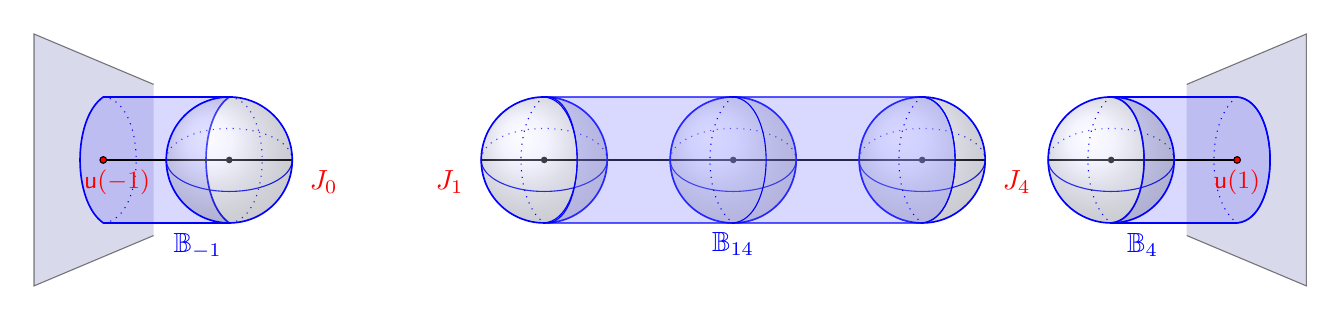
\begin{tikzpicture}[scale=0.8]
    \clip (-2.2,-2.1) rectangle (18.2,2.1);
    % boundary of M
    \fill[blue!50!black,opacity=0.15,draw=black,draw opacity=0.5]
        (16.2,-1.2) -- (18.1,-2) -- (18.1,2) --  (16.2,1.2) ;
    \fill[blue!50!black,opacity=0.15,draw=black,draw opacity=0.5]
        (-0.2,1.2) -- (-2.1,2) -- (-2.1,-2) -- (-0.2,-1.2) ;
    % cylinder left
    \fill[draw=blue,semithick,fill=blue!50!white,fill opacity=0.3]
        (-1,-1) -- (1,-1) to[out=145,in=-145, distance=0.6cm] 
        (1,1) -- (-1,1) to[out=-145,in=145, distance=0.6cm] (-1,-1);
    \draw[semithick,blue] 
        (-1,1) -- (1,1) 
        (1,-1) -- (-1,-1);
    % vertical arcs on the first sphere
    \foreach \x in {-1,1}{
        % \draw[blue,semithick]
        %     (\x,1) to[out=-145,in=145, distance=0.6cm] (\x,-1);
        \draw[blue, dotted]
            (\x,1) to[out=-5,in=5, distance=0.7cm] (\x,-1);
    }
    % right cylinder
    \fill[draw=blue,semithick,fill=blue!50!white,fill opacity=0.3]
        (15,1) -- (17,1) to[out=-5,in=5, distance=0.7cm] 
        (17,-1) -- (15,-1) to[out=5,in=-5, distance=0.7cm] (15,1);
    % old
    \draw[semithick]
        (-1,0) -- (2,0)
        node[pos=0.5, below=0.8cm,blue]{$\mathbb{B}_{-1}$}
        (5,0) -- (13,0)
        (14,0) -- (17,0) node[pos=0.5, below=0.8cm,blue]{$\mathbb{B}_{4}$}
        ;
    \draw[thick, red]
        (2.5,0) node[below]{$J_{0}$}
        (4.5,0) node[below]{$J_{1}$}
        (13.5,0) node[below]{$J_{4}$}
        % (16.5,0) node[below]{$J_{5}$}
        ;
    % \draw[mygreen, thick]
    %     (0,0) -- (2,0) node[fill=mygreen!20,draw, pos=0.5]{}
    %     (1, 0) node[below=2pt]{$J_0$};
    \foreach \y/\ytext in {1/0,6/1,9/2,12/3,15/4}{
        \fill[fill=black] (\y,0) circle (1.5pt) ;
    }
    %spheres
    \foreach \y in {1,6,9,12,15}{
        \draw[blue] (\y-1,0) arc (180:360:1cm and 0.5cm);
        \draw[blue,dotted] (\y-1,0) arc (180:0:1cm and 0.5cm);
        \shade[ball color=blue!20!,opacity=0.3] (\y,0) circle (1cm);
        \draw[blue,semithick] (\y,0) circle (1cm);
        }
    %blue cylinder
    \fill[draw=blue,fill=blue!50!white,fill opacity=0.3]
        (6,1) -- (12,1) to[out=-5,in=5, distance=0.7cm] (12,-1) -- (6,-1) to[out=-5,in=5, distance=0.7cm] (6,1);
    \draw[color=blue] (9, -1) node[below]{$\mathbb{B}_{14}$};
    % vertical arcs
    \foreach \x in {6,9,12,15,17}{
        \draw[blue]
            (\x,1) to[out=-5,in=5, distance=0.7cm] (\x,-1);
        \draw[blue,dotted]
            (\x,1) to[out=-145,in=145, distance=0.6cm] (\x,-1);
    }
    % \foreach \y in {0,2}{
    %     \fill[mygreen,draw=black,semithick] (\y,0) circle (1.5pt);
    % }
    \fill[red,draw=black]
        (-1,0) circle (1.5pt) (-0.78,0) node[below]{\small$\mathsf{u}({-}1)$}
        (17,0) circle (1.5pt) node[below]{\small$\mathsf{u}(1)$};
\end{tikzpicture}
\end{tabular}
\end{document}